\documentclass{beamer}

% ---- PACKAGES ----
\usepackage[francais]{babel}
\usepackage[T1]{fontenc}
\usepackage[utf8]{inputenc}

% ---- THEME ----
\usetheme{Dresden}
\usecolortheme{beaver}

% ---- PAGE NUMBER ----
\setbeamertemplate{footline}%{miniframes theme}
{%
	\begin{beamercolorbox}[colsep=1.5pt]{upper separation line foot}
	\end{beamercolorbox}
	\begin{beamercolorbox}[ht=2.5ex,dp=1.125ex,%
		leftskip=.3cm,rightskip=.3cm plus1fil]{author in head/foot}%
		\leavevmode{\usebeamerfont{author in head/foot}\insertshortauthor}%
		\hfill%
		{\usebeamerfont{institute in head/foot}\usebeamercolor[fg]{institute in head/foot}\insertshortinstitute}%
	\end{beamercolorbox}%
	\begin{beamercolorbox}[ht=2.5ex,dp=1.125ex,%
		leftskip=.3cm,rightskip=.3cm plus1fil]{title in head/foot}%
		{\usebeamerfont{title in head/foot}\insertshorttitle} \hfill     \insertframenumber%
	\end{beamercolorbox}%
	\begin{beamercolorbox}[colsep=1.5pt]{lower separation line foot}
	\end{beamercolorbox}
}

% ---- TITLE PAGE DECLARATION ----
\title[Hel : The pixelated horror]{Hel : The pixelated horror}
\subtitle{Travail de diplôme 2015}
\author{Yannick R. Brodard}
\institute{Centre de Formation Professionnelle Technique\\École d'informatique}
\date{Mercredi, 10 juin 2015}
\subject{Informatique}

% ---- DOCUMENT BEGINNING ----
\begin{document}
\frame{\titlepage}

% ---- TABLE OF CONTENTS
\begin{frame}
\frametitle{Sommaire}
\tableofcontents[hideallsubsections]
\end{frame}

%\AtBeginSection[]
%{
%  \begin{frame}
%    \frametitle{Sommaire}
%    \tableofcontents[currentsection,hideallsubsections]
%  \end{frame}
%}

% ---- CONTEXTE DU PROJET ----
\section{Introduction}
\subsection{}
\begin{frame}
\begin{columns}
\column{0.5\textwidth}
	\begin{itemize}
		\item Jeu-vidéo 2D
		\item Aspects RPG
		\begin{itemize}
			\item Système de compétences
			\item Système d'objets
		\end{itemize}
		\item Monogame
	\end{itemize}
\column{0.5\textwidth}
\begin{figure}
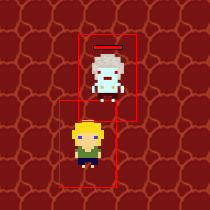
\includegraphics[width=1\textwidth]{img/hitbox.png}
\end{figure}
\end{columns}
\end{frame}

\begin{frame}
\begin{columns}
\frametitle{Pourquoi ce sujet ?}
\column{0.5\textwidth}
\begin{itemize}
	\item Les jeux ressemblants sont :
	\begin{itemize}
		\item Trop faciles
		\item ou trop complexes
	\end{itemize}
	\item Trouver le juste milieu
	\item Défi à soi-même
\end{itemize}
\column{0.5\textwidth}
\begin{center}

\includegraphics[width=0.45\textwidth]{img/pres_diablo3.png}\\

\includegraphics[width=0.45\textwidth]{img/pres_poe.png}\\

\includegraphics[width=0.45\textwidth]{img/pres_bastion.png}
\end{center}
\end{columns}
\end{frame}

% ---- HEL ET ENVIRONNEMENT
\begin{frame}
\frametitle{Hel et son histoire}
\begin{columns}
\column{0.5\textwidth}
\begin{itemize}
	\item Basé sur la mythologie nordique
	\item Hel, déesse de la mort
\end{itemize}
\column{0.5\textwidth}
\begin{center}
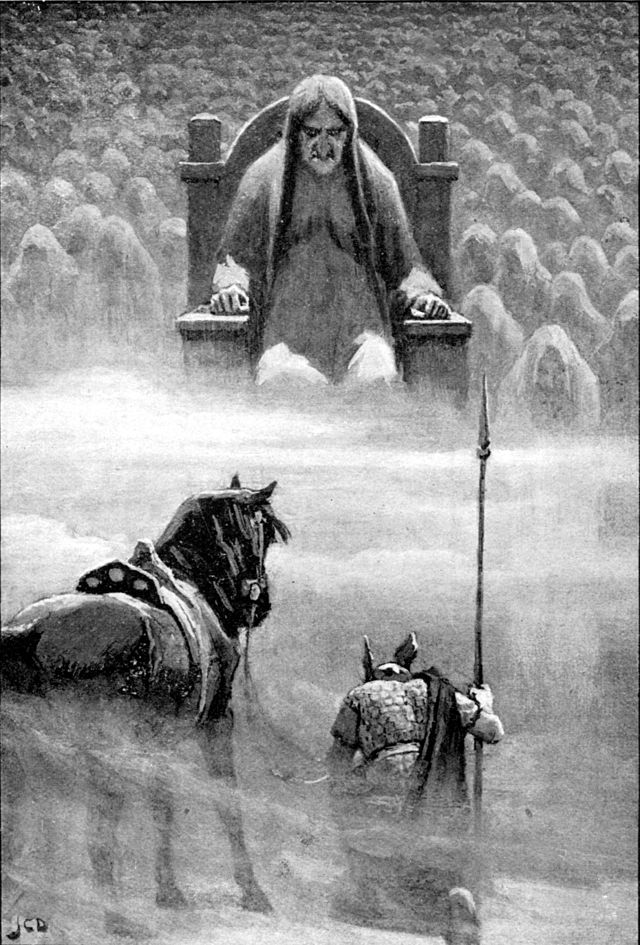
\includegraphics[width=.75\textwidth]{img/Hel_goddess_of_death.jpg}
\end{center}
\end{columns}
\end{frame}

% ---- FONCTIONNALITÉS ----
\section{Fonctionnalités}
\subsection{}

% ---- MONOGAME ----
\begin{frame}
\begin{columns}
\column{0.5\textwidth}
\begin{itemize}
	\item Boucle de jeu
	\item Gestion des textures
	\item Gestion de l'affichage
	\item Utilisation du GPU
\end{itemize}
\column{0.5\textwidth}
\begin{center}

\includegraphics[width=.75\textwidth]{img/pres_monogame_logo.png}
\end{center}
\end{columns}
\end{frame}

\begin{frame}
\begin{center}
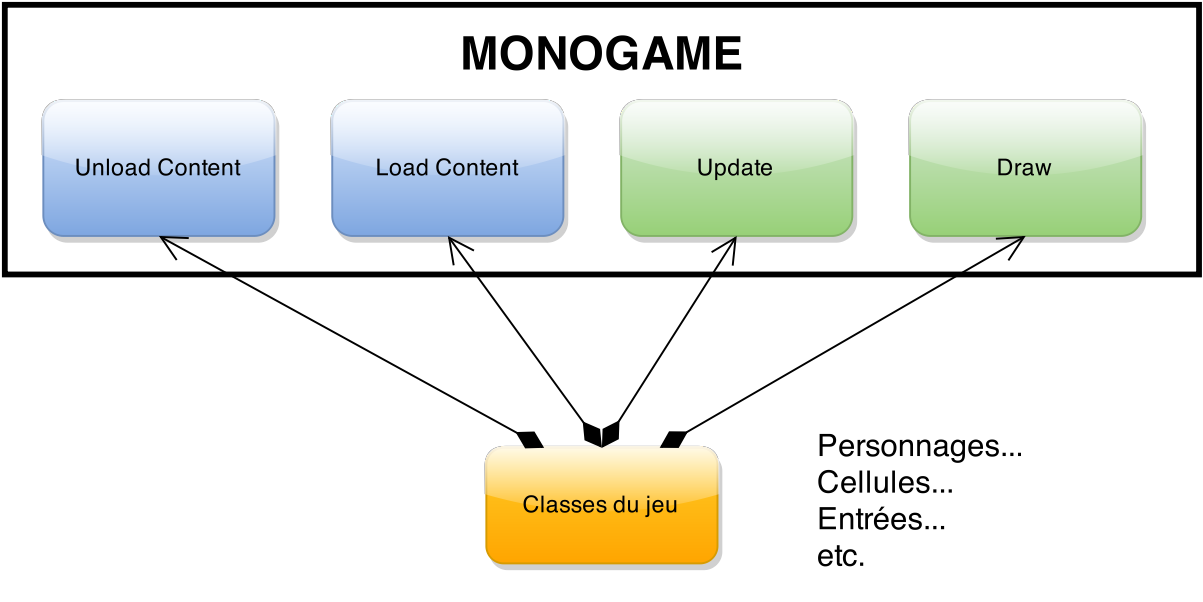
\includegraphics[width=.85\textwidth]{img/pres_boucles.png}\\
\end{center}
\end{frame}

% ---- OUTILS ----
\begin{frame}
\frametitle{Outils de développement}
\begin{columns}
\column{0.5\textwidth}
\begin{itemize}
	\item Primitives 2D
	\item Collisions/intersections
	\item Gestion des entrées
	\item Sérialisation XML
\end{itemize}
\column{0.5\textwidth}
\begin{center}

\includegraphics[width=0.5\textwidth]{img/pres_prim2d.png}\\

\includegraphics[width=0.5\textwidth]{img/pres_keys.jpg}\\
\end{center}
\end{columns}
\end{frame}

\begin{frame}
\begin{center}
\begin{figure}
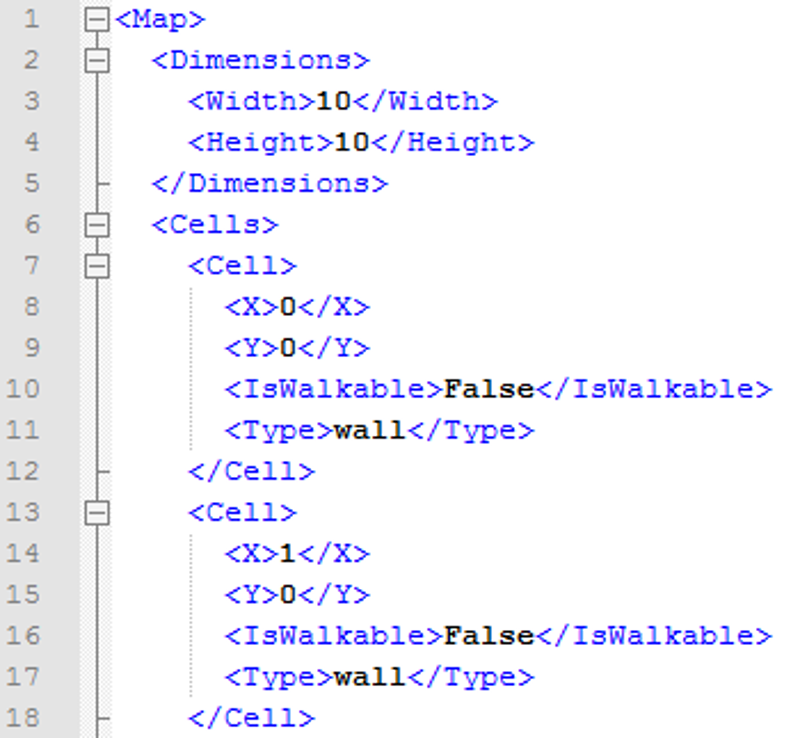
\includegraphics[width=0.65\textwidth]{img/pres_xml.png}
\caption{Fichier XML du village}
\end{figure}
\end{center}
\end{frame}

\begin{frame}
Le jeu possède :
\begin{itemize}
	\item Des règles de jeu
	\item Une carte générée aléatoirement
	\item Un personnage contrôlable
	\item Des ennemis indépendants
\end{itemize}
\end{frame}

\begin{frame}
\frametitle{Règles du jeu}
\begin{columns}
\column{0.5\textwidth}
\begin{itemize}
	\item Vaincre des ennemis
	\item Gagner des points de compétences
	\item Trouver des objets
	\item Vaincre le boss "Hel"
\end{itemize}
\column{0.5\textwidth}
\begin{center}

\includegraphics[width=.45\textwidth]{img/pres_strenght.png}\\

\includegraphics[width=.45\textwidth]{img/pres_vitality.png}\\

\includegraphics[width=.45\textwidth]{img/pres_agility.png}\\

\includegraphics[width=.45\textwidth]{img/pres_magic.png}
\end{center}
\end{columns}
\end{frame}

% ---- MÉTHODES MISES EN OEUVRE ----
\section{Méthodes}
\subsection{}

\begin{frame}
\frametitle{Carte}
\begin{columns}
\column{0.5\textwidth}
\begin{itemize}
	\item Génération aléatoire
	\item Utilise un algorithme d'automate cellulaire
	\begin{itemize}
		\item Réagi selon les voisins
	\end{itemize}
\end{itemize}
\column{0.5\textwidth}
\begin{center}
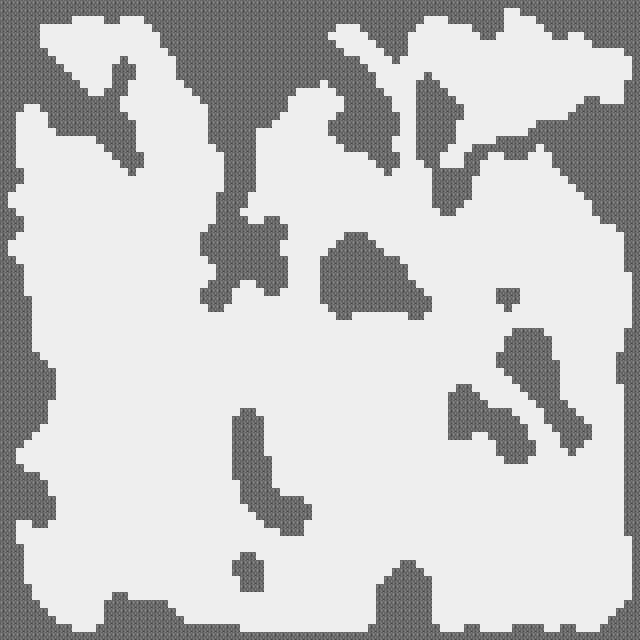
\includegraphics[width=1\textwidth]{img/map_example.png}\\
\end{center}
\end{columns}
\end{frame}

\begin{frame}
\frametitle{Les éléments du jeu}
\begin{center}
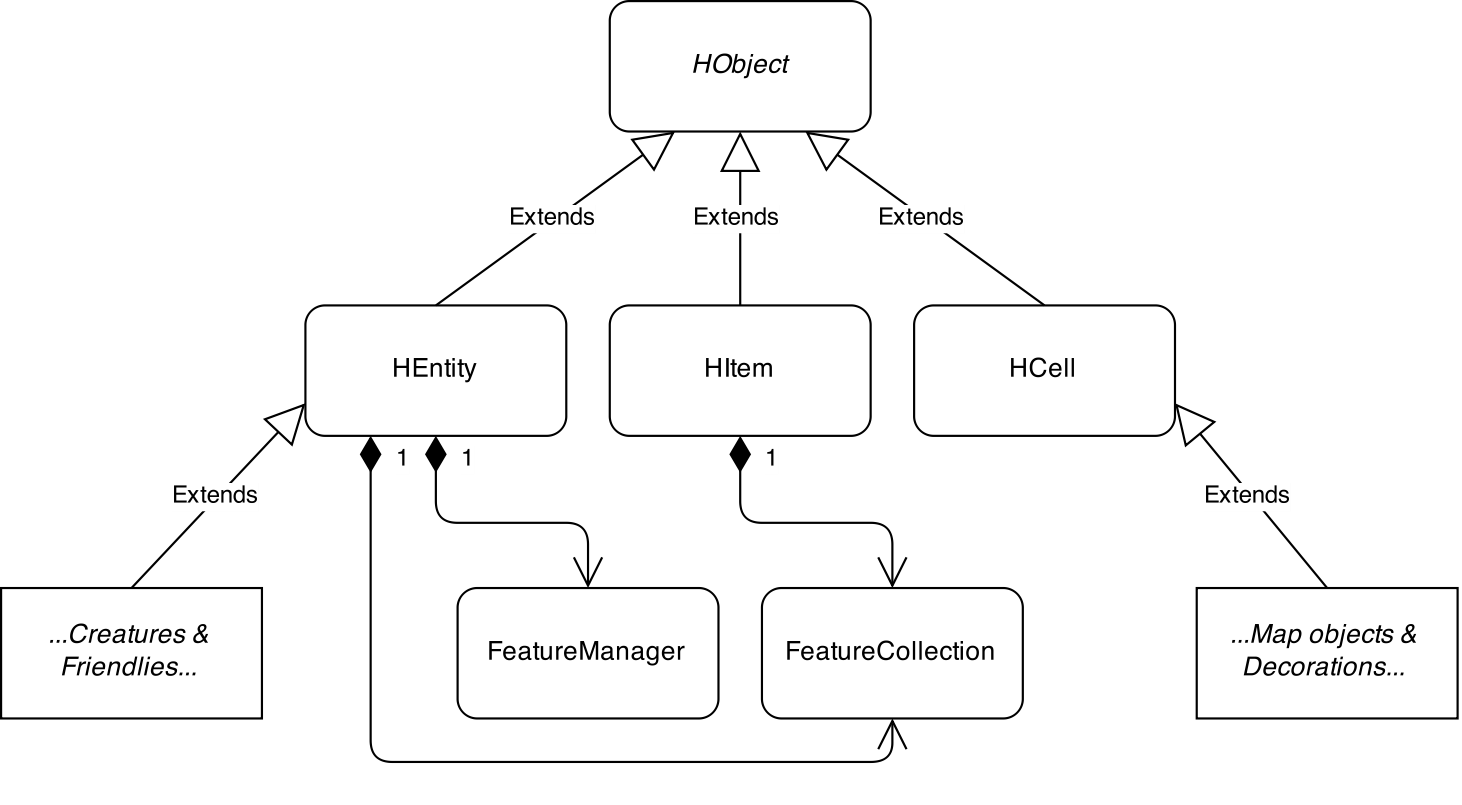
\includegraphics[width=1\textwidth]{img/WorldObjects.png}
\end{center}
\end{frame}
	
\begin{frame}
\begin{center}
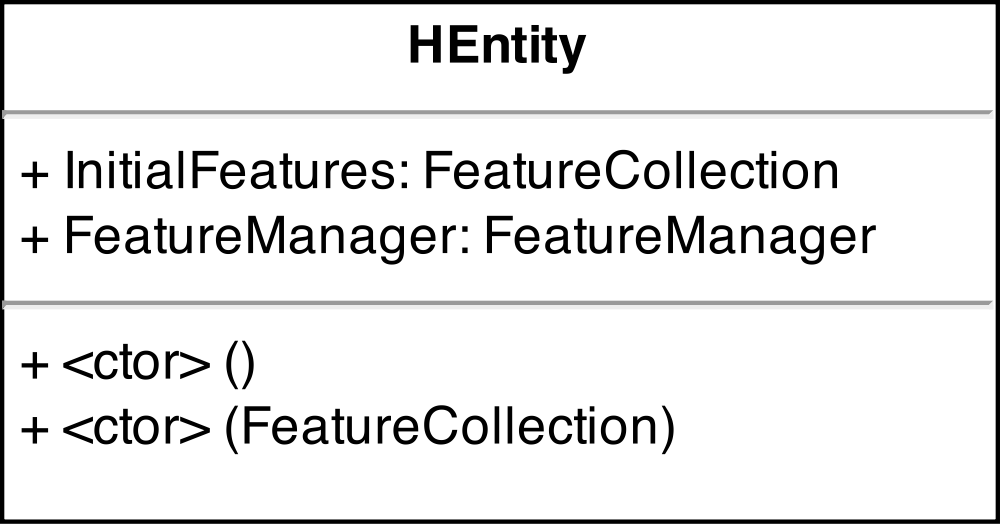
\includegraphics[width=0.69\textwidth]{img/HEntity.png}
\end{center}
\end{frame}


% ---- DEMONSTRATION ----
\section{Démonstration}
\subsection{}
\begin{frame}
\begin{center}

\includegraphics[width=0.5\textwidth]{img/pres_demo.png}
\end{center}
\end{frame}

% ---- CONCLUSION ET PERPECTIVES ----
\section{Conclusion}
\subsection{}
\begin{frame}
\begin{itemize}
\item Conclusion
\begin{itemize}
	\item Terminer le système d'objets et de points de compétences.
	\item Ajout de contenu est simple
	\item Nécessite beaucoup de temps de travail
\end{itemize}
\item Perspectives
\begin{itemize}
	\item Une version stable d'ici quelques mois
	\item Peut être suivi sur GitHub : \url{www.github.com/brodardy}
\end{itemize}
\end{itemize}
\end{frame}

\begin{frame}
\frametitle{Questions ?}
\begin{center}

\includegraphics[width=0.25\textwidth]{img/question.png}
\end{center}
\end{frame}
\end{document}